\begin{savequote}[75mm] 
She a pretty penny and she know I'm doing numbers\\
Till we crash up the whole database
\qauthor{``Paradise''- Big Sean } 
\end{savequote}

\chapter{Data}

\section{Sources}
We used influence and audio data from AllMusic\footnote{\url{https://www.allmusic.com/}}, cover song data from SecondHandSongs\footnote{\url{https://secondhandsongs.com/}}, and collaboration data from MusicBrainz\footnote{\url{https://musicbrainz.org/}}. Additionally, song release year information was queried for via Discogs\footnote{\url{https://www.discogs.com/}}.

\subsection{AllMusic}
True to its name, AllMusic is the largest music database on the web, cataloging information on over 3 million albums and 30 million tracks, along with associated artist information and other metadata.

AllMusic maintains individual Artist pages, which among other information includes human-curated data on a particular artist's \textit{influencers} (denoted as ``Influenced By'') and \textit{followers} (denoted as ``Followed By''). The site defines influencers as ``Artists that have had a direct musical influence on, or were an inspiration to, the selected artist, as determined by our music editors'' and followers as ``Artists who were influenced by the selected artist. This may be directly called  from research and interviews, or it may be a strong inference based on the opinion of the editors'' \footnote{\url{https://www.allmusic.com/faq}}.

\begin{figure}[H]
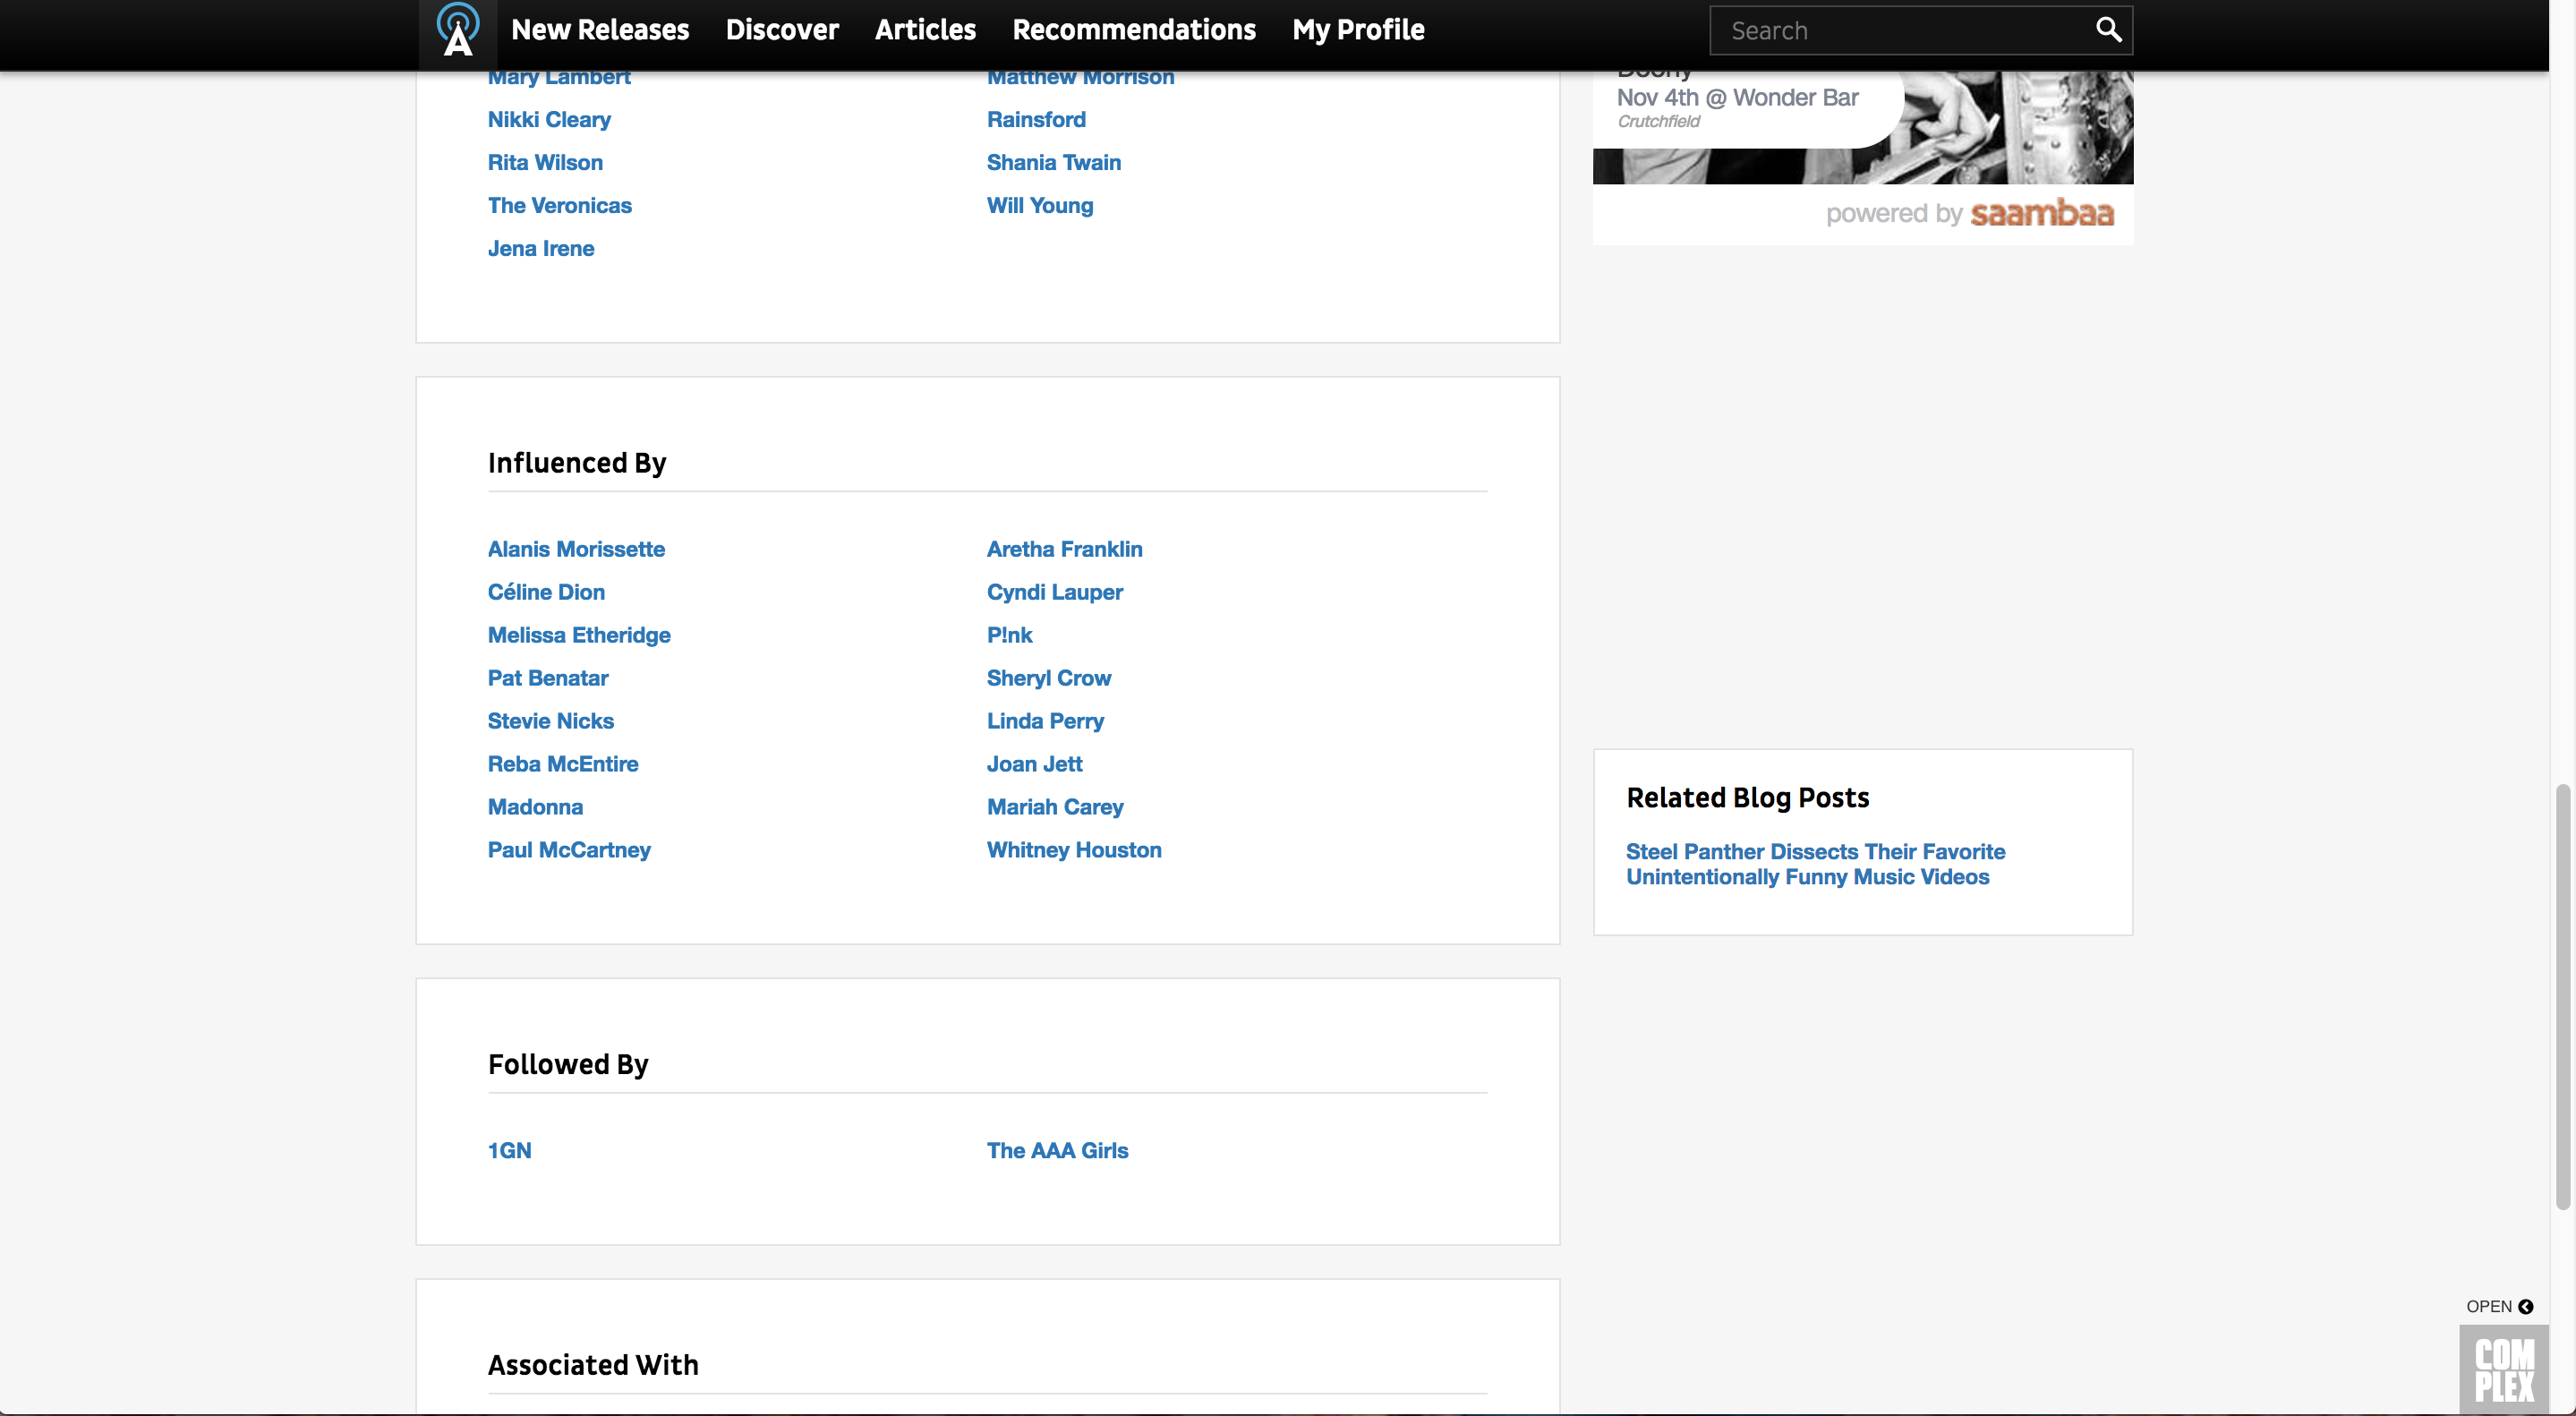
\includegraphics[width=\textwidth]{figures/allmusic_influences.png}
\caption{Example of influencers and followers for an Artist on AllMusic}
\end{figure}

In addition to textual metadata, AllMusic also includes audio data in the form of a series of several (up to 10) 30 second long previews of songs recorded by a particular Artist. 

\subsection{SecondHandSongs}
SecondHandSongs (SHS) is a cover songs database with an emphasis on data quality. For each original work, the site maintains information on the original recording and known subsequent versions recorded by other artists, commonly referred to as \textit{covers}. Each cover has information on the performer that recorded the work along with the release date of the cover. Visitors to the site can post suggestions for new covers, but each version is verified by a human editor prior to inclusion in the database.

\begin{figure}[H]
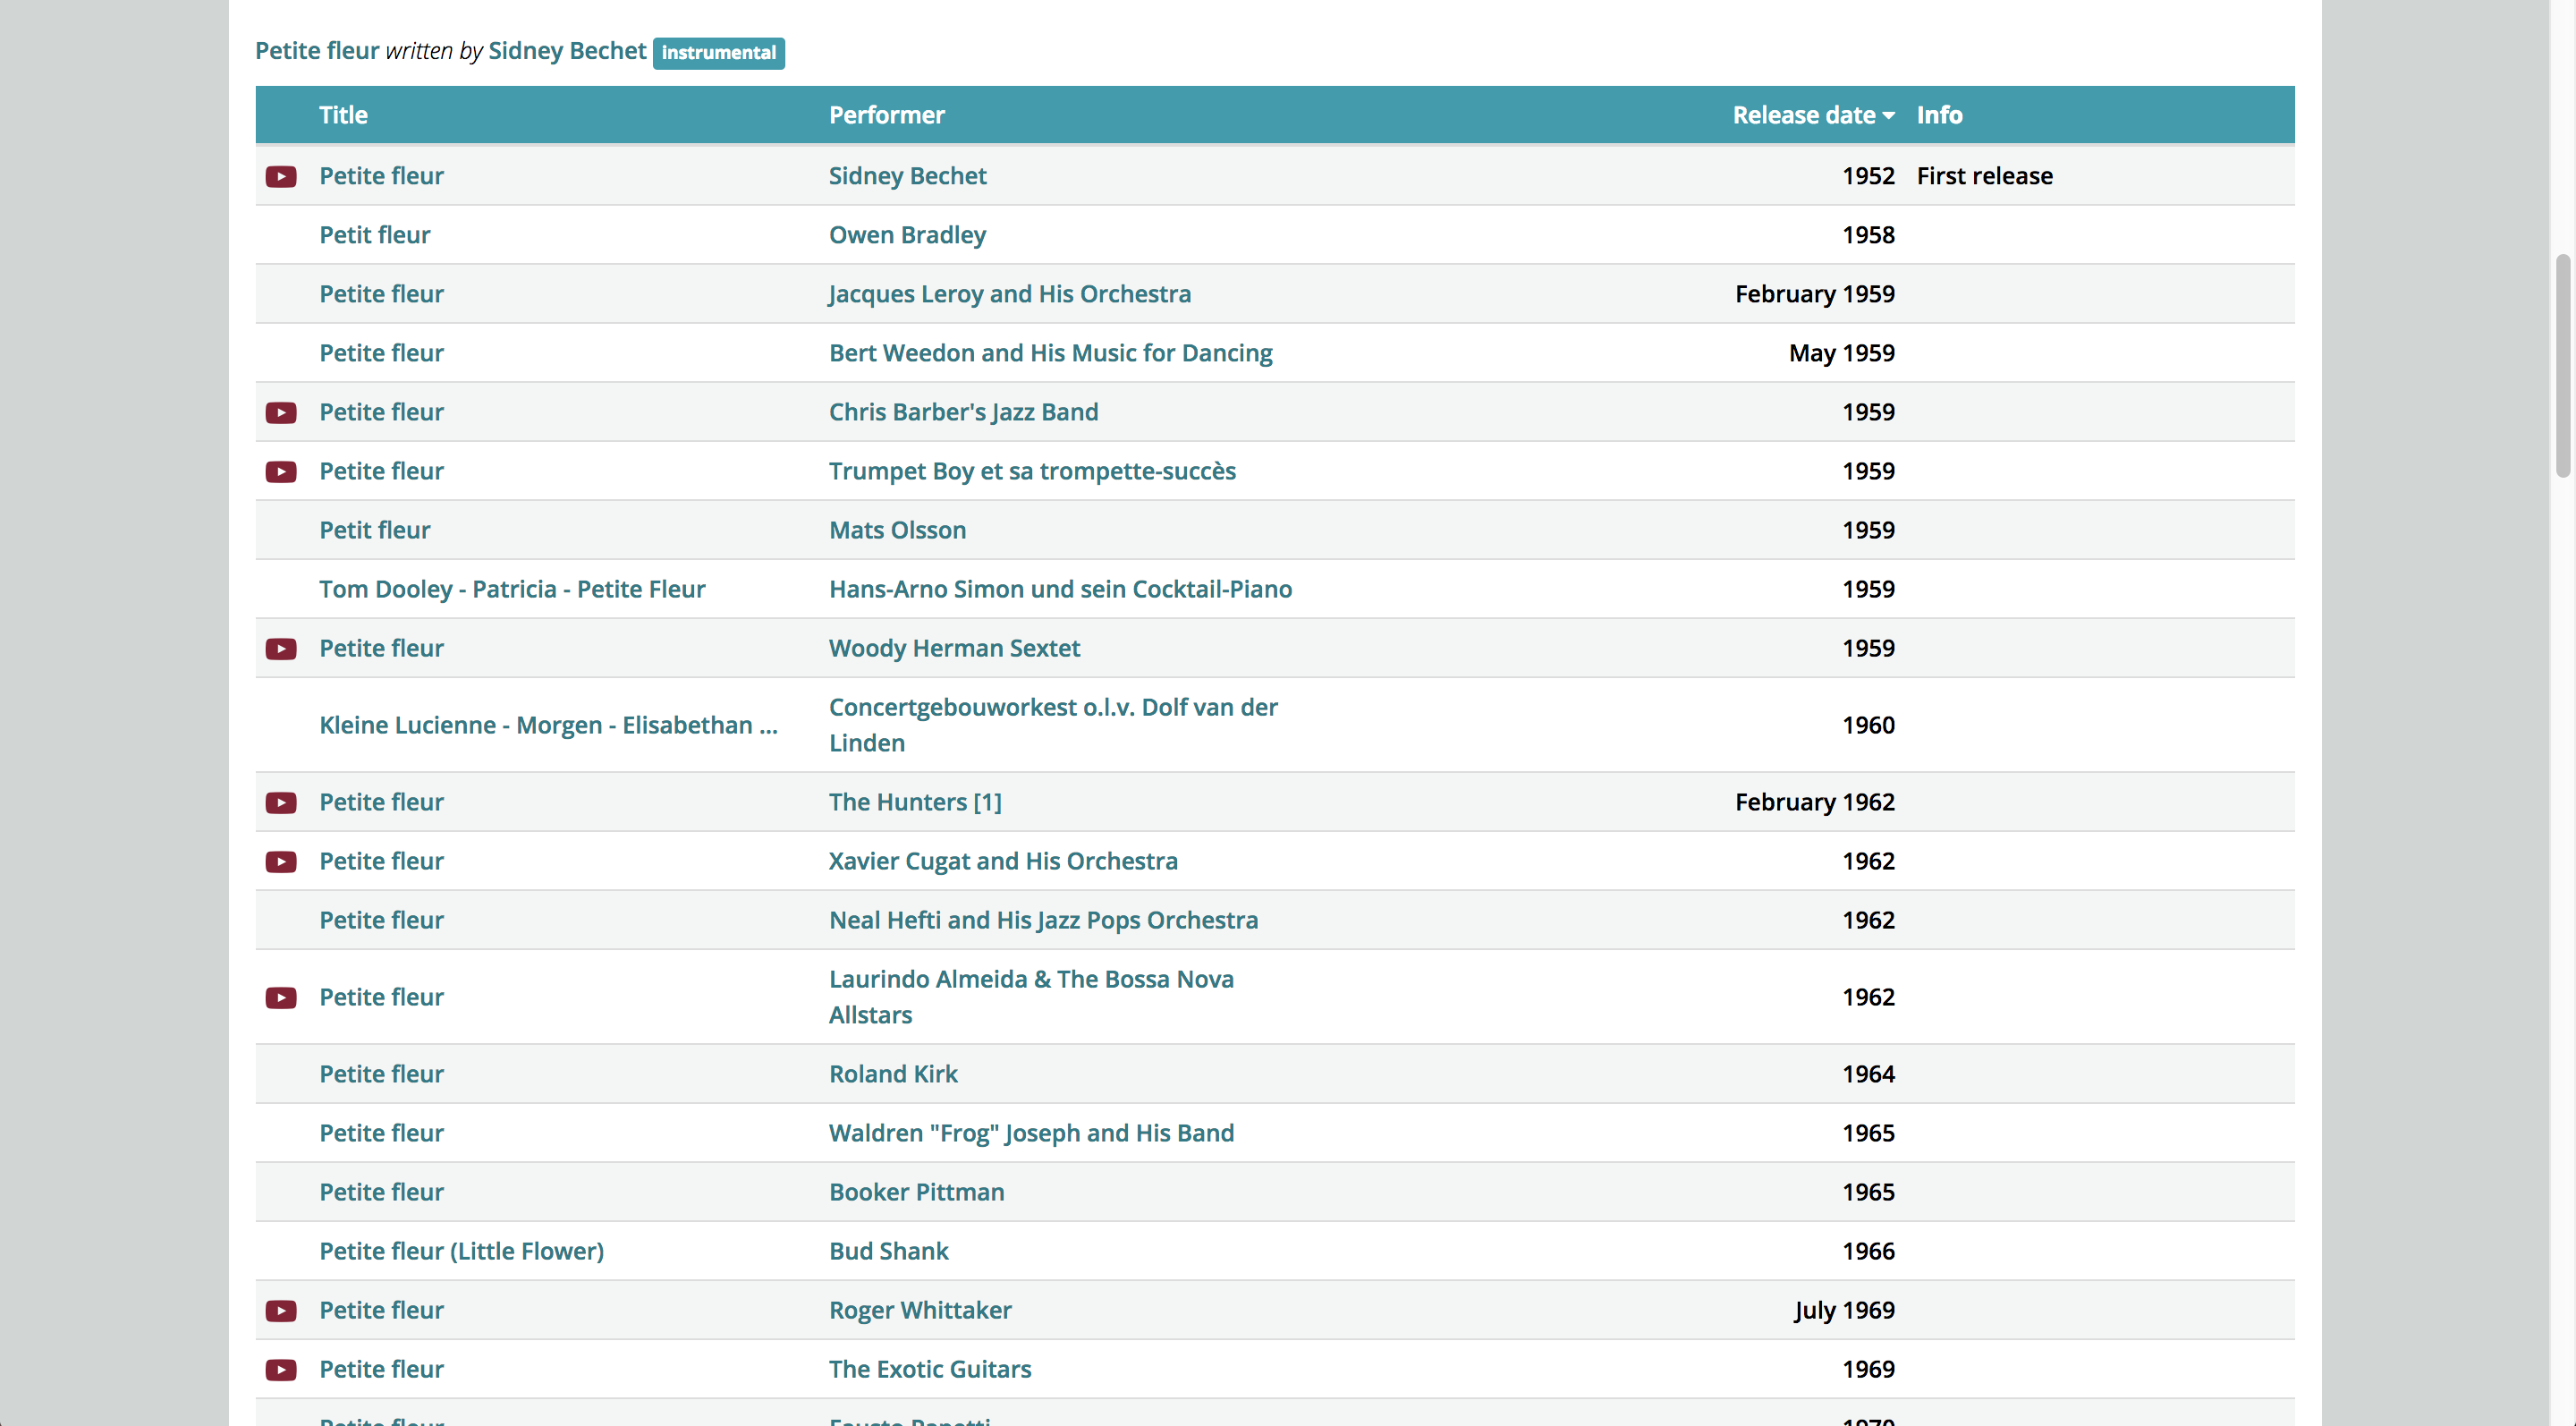
\includegraphics[width=\textwidth]{figures/shs_example.png}
\caption{Example of cover versions for a song on SecondHandSongs}
\end{figure}

\subsection{MusicBrainz}
MusicBrainz is an open database of music metadata on artists and recordings. While the database is quite extensive, we used it for the limited purpose of extracting collaboration relationships between musicians. In this case, two artists are said to have collaborated if there exists a recording on which the artists are both listed within the MusicBrainz database.

\subsection{Discogs}
Discogs is a crowdsourced database about audio recordings, with information on over 9 million releases by over 5 million artists. Though accuracy is a concern because of the nature of crowdsourcing, due to its easy-to-use public API, we used Discogs in order to collect song release year information.

\section{Collection}
\subsection*{Scraping AllMusic}
Since AllMusic does not have a free public API, we scraped influence information from the website directly. AllMusic provides a link to the respective Artist pages of the influencers and followers of a given Artist, which enabled us to construct a directed graph of influence relationships via breadth-first search (BFS). 

We started on the Artist page of the jazz saxophonist Charlie Parker, adding a directed edge leading to Charlie Parker for each of his influencers and a directed edge leading away from Charlie Parker for each of his followers. We then added the associated Artist page URLs of each of the influencers and followers to a queue for exploration via BFS. When visiting each Artist page, we additionally collected metadata on the artist visible on the page, namely the active period of their career (i.e. 1930s - 1950s for Charlie Parker), and associated genres and styles.

A natural assumption of this approach is that starting the breadth-first search from Charlie Parker covers a sufficient number of genres and periods of influence relationships. This assumption is reasonable, given that our approach generated over 90,000 influence relationships between over 16,000 artists spanning genres including jazz, rock, country, classical, electronic, rap and pop and periods dating from the early 20th century to the present day. That said, a caveat is that since BFS from a single initial node necessarily yields a single weakly connected component, any influence relationships not connected to this component will be missing in our data.

We also collected audio data from AllMusic. Using the unique identifiers for each artist obtained during the scraping of influence relationships, we scraped AllMusic once again for available audio clips of songs by the artist. Since the number of audio clips we needed to scrape was much larger than the number of Artist pages visited during the initial BFS scraping process, we distributed audio scraping between multiple machines on Amazon Web Services (AWS).

\subsection*{Scraping SecondHandSongs}
SecondHandSongs has a public facing API, but unfortunately the API does not return recording date information, which was essential for our purposes. Therefore we scraped the individual Work pages from the website in order to have access to the sequence of covering artists and cover release dates for each original musical work. Since each work page on SHS is indexed numerically by id (i.e. \url{https://secondhandsongs.com/work/<id>}), we queried all ids between 1 and 200000 (since not all ids are yet defined), distributing the scraping process between multiple machines on AWS.

\subsection*{MusicBrainz Collaboration Data}
An undirected graph of collaboration relationships between musicians who made a recording together in the MusicBrainz database has previously been constructed\footnote{\url{https://github.com/basimr/snoop-dogg-number/tree/master/graph}}, so we used it directly.

\subsection*{Querying the Discogs API for Release Year Information}
Discogs exposes a public API for requesting song metadata from its database. Using this API we were able to fuzzy search for song release year based on artist name and song name, as there was no way to access this information from AllMusic.com directly for the audio that we scraped. In total, we were able to collect release year information for 126024 songs out of 138008 total, obtaining 91\% coverage. 
